\subsection{介质对晶体生长的影响}
% OCR Product
% To be fixed
实际晶体都是在一定的介质环境中生长的,因此介质必然对晶体(外形和完整性)发生影响,开展这方面的研究,不仅对于培养优质单晶,而且对于探讨实际晶体的形成问题都具有重要的意义,介质对从溶液中生长晶体的影响主要包括以下几个因素:杂质、溶液中氢离子浓度(pH值)、温度、过饱和度和介质运动等。

\paragraph{(1)杂质}通常把与结晶物质无关的少量外来物质称为杂质。杂质在结晶过程中一般是难以避免的。广义的杂质还应该包括溶剂本身,从这个意义上来说,杂质是不能消除的(其含量有时甚至是很大的),因为它本身就是外介质。

杂质对晶体生长的影响是多方面的,研究杂质效应不仅有助于控制结晶过程和单晶的性质,而且在晶体生长理论研究上也有重要的作用,因为杂质影响的机制常与晶体生长动力学的研究紧密联系在一起的。

杂质可以影响溶解度和溶液的性质,例如在生长某些晶体时,常在溶剂中加入一定量(百分之几)的辅助剂或使用混合溶剂,以改变溶解度或溶液的粘度,使有利于晶体的生长(表3.10)。

(表3.10)

杂质也会显著地改变晶体的结晶习性(晶癖),Buckley曾用许多篇幅对此作了专门叙述,在工业结晶中也常应用杂质这一效应,表3.11列出了其中的一些典型例子。

(表3.11)

杂质对晶体质量也有明显的影响。在多数情况下,杂质使晶体的完整性降低,性能变坏,但也存在一些少量杂质离子能改善晶体生长质量,其侧子见表3.12。有时为了改善晶体某一方面的性能,还需加入一些杂质(掺质)。例如在TGS晶体中掺入$\alpha$丙氨酸以防止退极化。

(表3.12)

杂质影响晶体生长有以下三种方式:
\begin{enumerate}[(i)]\itemsep -0.5ex
\item 进入晶体;
\item 选样性吸附在一定的晶面上;
\item 改变晶面对介质的表面能,
\end{enumerate}

杂质进入晶体的机制井不十分清楚,一般来说,由于结晶作用的专一性,生长中的晶体对外来杂质有排斥作用。但有时晶体表面也可以键合杂质质点,特别是它与组成晶体的质点在晶体构造中较为相似时,比较容易均匀地进人晶体,相似性愈大,进入晶体就愈容易,例如在生长DKDP晶体时,H就可以进入D的位置,形成均匀的$\rm K(D_xH_{1-x})_2PO_4$混晶。在掺$\alpha$丙氨酸的TGS晶体(称ATGS)中,$\alpha$丙氨酸之所以能进入TGS晶格中,主要是由于$\alpha$丙氨酸分子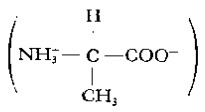
\includegraphics[height=10ex]{fig/cp03/fml4.1.jpg}和甘氨酸分子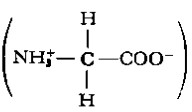
\includegraphics[height=10ex]{fig/cp03/fml4.2.jpg}在结构上的相似性。杂质的这种均匀进入通常会对晶体的性质发生影响。当然,这种进入一般是有一定限度的,超过这一限度常会引起晶体构造的不稳定。有时杂质(包括溶剂)也会不均匀地进入晶体,造成包裹物,这主要是由外因引起,如过饱和度过大,溶液搅拌不均匀等。

由于晶体的各向异性,杂质在晶体的不同晶面上经常发生选择性吸附。这种吸附常使某些晶面的生长受到阻碍,因而改变了各晶面的相对生长速度。在杂质改变晶癖的例子中有不少是由这种原因造成的。选择性吸附还普遍具有饱和性,即当溶液中杂质含量超过一定浓度后,它对生长的遏制作用不再随杂质浓度的增大而增长。选择性吸附对晶体的影响方式以进入晶体为主。如在含有$\rm CuCO_3$的溶液中生长KTN晶体时,$\rm Cu^{2+}$只吸附在\{001\}晶面上,阻碍其生长,但对[001]晶带上的晶面却无影响,结果使KTN晶体$Z$向变短,甚至呈板状。\{001\}表层呈深蓝色,说明$\rm Cu^{2+}$已进入了<001>的生长锥。

必须指出,同一种晶面对不同杂质离子或同一种离子对不同晶面选择性吸附影响的程度是很不相同的。例如三价金属离子$\rm Cr^{3+}$,$\rm Fe^{3+}$,$\rm Al^{3+}$很容易在KDP型晶体的柱面上发生选择性吸附,使柱面楔化(图3.37),但其楔化能力却不一样,在相同的杂质浓度下,按$\rm Cr^{3+}>Fe^{3+}>Al^{3+}$递降。这可能与相应水合离子$\rm M(H_2O)_6^{3+}$的稳定性有关,因其稳定性递减次序恰好是$\rm Cr(H_2O)_6^{3+}>Fe(H_2O)_6^{3+}>Al(H_2O)_6^{3+}$。微量的$\rm Cr^{3+}$很容易进入晶体柱面的生长扇形,使此部分呈绿色[图3.37(c)]。

三价金属离子在KDP型晶体柱面上发生选择性吸附,常常使晶体柱面楔化,光学均匀性降低,这固然是其有害的一面,但也有其可利用的一面。在培养大块晶体时,人们按预定的要求 用规定尺寸横截面的种子,不希望横截面再扩大,而在纯度较高的溶液中生长此类晶体横截面会扩大,有时甚至达到无法控制的程度,使光轴方向生长达不到要求的尺寸,为此必须抑制晶体柱面生长,加入一定量有选择性吸附能力的三价金属离子可以实现上述目标。有趣的是,加入三价金属离子后,溶液的准稳区扩大,稳定性大大提高,而柱面上产生的楔化度可通过加大过饱和度得到补偿(图3.31),使KDP型晶体在$Z$向上的生长速度大大提高。


\begin{figure}[htbp]
 \centering
 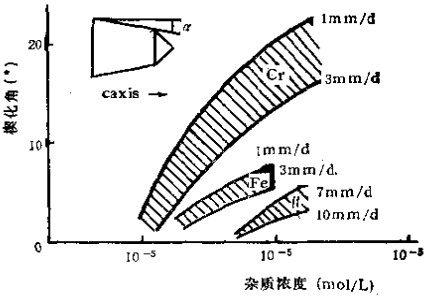
\includegraphics[width=0.8\textwidth]{fig/cp03/img3.31.jpg}
 \caption{杂质浓度和楔化角间关系;楔化角与生长速度的函数关系。}
\end{figure}

杂质改变了晶面对介质的表面能,从晶体生长的分子动力学理论来看,这可以看成时改变各种生长过程的能量。如果杂质不进入晶体,只是在溶液中和溶质相互作用,那么只能均匀地改变所有质点的结合能,表现为杂质对溶解度和晶体生长速度的影响。如果杂质进入晶体,则晶格场受到局部破坏。杂质在不同晶面上进入的情况是不一样的,对各个晶面上质点结合能影响的程度也是不相同的,其结果就是改变了各晶面的相对生长速度。

综上所述,杂质的影响包括晶体学、动力学和热力学等方面的效应,影响的主要方式是进入晶体。


\paragraph{(2)氢离子浓度(pH)}在水溶液中存在着大量的$\rm H^+$和$\rm OH^-$,溶液中的氢离子浓度对晶体生长的影响是很显著的。例如提高溶液的pH值会促使KDP型晶体柱面扩展,降低pH值使得LSH和TGS晶体发育较为匀称。如果溶液pH值不合适,即便是其它生长条件合适,也长不出所需尺寸的好晶体。pH影响也是相当复杂的,一般可归纳为以下几种方式:
\begin{enumerate}[(i)]\itemsep -0.5ex
\item pH影响溶解度,使溶液中离子平衡发生变化。
\item pH改变杂质的活性,即改变杂质络合或水合状态,使杂质敏化或钝化。pH的作用也可能改变晶面的吸附能力,因pH对后者有较大的影响。
\item pH直接影响晶体生长,通过改变各晶面的相对生长速度,引起晶体生长习性的变化。例如25摄氏度时,在$\rm pH=3.8$的溶液中,ADP晶体在$X$方向上生长速度为0,晶体沿$Z$方向伸长。当$\rm pH=5.2$时,沿$Z$向生长速度增长不多,但$X$向生长速度却有明显的增加,晶体长成较短的棱柱体(图3.32)。Mullin把$\rm H^+$也看成和$\rm M^{3+}$一样的杂质离子来解释pH的影响机制:溶液中$\rm H^+$以水合离子$\rm H_3(H_2O)_3^+$存在,它在ADP柱面附近表现出稀释效应,阻碍溶质向晶面上扩散,因而遏制了该面生长。当pH升高时,氢离子浓度减小,阻碍作用减弱,柱面生长速度就增加了。
\end{enumerate}


\paragraph{(3)温度}生长温度对晶体的习性和质量都有影响。图3.33示出过饱和度相同、但生长温度不同的$\rm MgSO_4\cdot 7H_2O$晶体的习性变化。因此,可以利用晶体生长习性随温度的变化,选择合适的生长温度以获得所需要的晶癖。

温度本身的影响可以认为是改变晶体生长各个过程的激活能。晶体生长过程很少是纯表面反应或是扩散过程。一般在较低温度下,结晶过程主要由表面反应这一步控制。当温度升高时,生长速度加快,扩散就逐渐成为控制结晶过程的主要步骤了。在较高的温度下生长的晶体,由于结晶质点排斥外来杂质能力的增强,其长出的晶体质量一般要比在较低温度下生长的好些。


\begin{figure}[htbp]
 \centering
 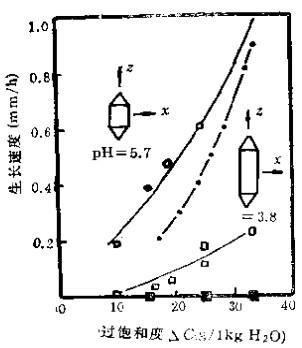
\includegraphics[width=0.8\textwidth]{fig/cp03/img3.32.jpg}
 \caption{pH对ADP晶体$X$和$Z$向生长速度的影响(25℃)。图中:}
$\bigcirc$为$\rm pH=5.2$时,$Z$向生长速度;\\
$\square$为$\rm pH=5.2$时,$X$向生长速度;\\
$\bullet$为$\rm pH=3.8$时,$Z$向生长速度;\\
$\blacksquare$为$\rm pH=3.8$时,$X$向生长速度。\\
\end{figure}

\begin{figure}[htbp]
 \centering
 \subfigure[25℃]{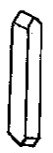
\includegraphics[height=24ex]{fig/cp03/img3.33a.jpg}}
 \subfigure[35℃]{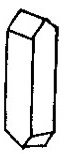
\includegraphics[height=24ex]{fig/cp03/img3.33b.jpg}}
 \subfigure[45℃]{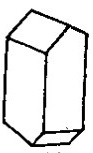
\includegraphics[height=24ex]{fig/cp03/img3.33c.jpg}}
 
 \caption{温度对$\rm MgSO_4\cdot 7H_2O$晶体外形的影响。}

\end{figure}

如果从结晶质点和介质的相互作用这一观点来研究实际晶体的形成过程时,可以把温度的影响看成是溶剂浓度的变化的影响(如果把溶剂看成杂质,也可以归结于杂质变化的影响)


\paragraph{(4)过饱和度和介质运动}过饱和度是结晶的驱动力,由于不同过饱和度会产生不同的生长机制,过饱和度对晶体生长速度、质量和晶体外形影响都很大。晶体在低过饱和度下生长时,速度较慢,晶面发展比较充分,一些高指数的次要晶面容易出露,ADP、KDP等晶体在过饱和度很低时,也会出现类似于杂质离子所造成的柱面楔化现象(图3.37),随着过饱和度的增加,楔化逐渐减轻到最后消失,经过这样的过程生长的晶体并不产生母液包藏。这种在很低过饱和度下出现的生长现象,可能是由于结晶驱动力过小、扩散到柱面附近的溶质质点无力穿过柱面-锥面交界处的“水分子壁垒”所造成的。用放射自显影术研究铁离子在KDP晶体中的分配的实验结果也表明,适当增加过饱和度(在较小的过饱和度范围内)有助于减少铁离子在柱面上的进入。

控制过饱和度是控制溶液晶体生长速度和质量的关键措施。大的过饱和度有利于晶体的自提纯作用和晶形简化,使晶体光学均匀性变好,而生长速度又快。但大的饱和度容易造成晶面上各部分过饱和度差变大,特别是大晶面,容易出现由于生长速度上的差异造成母液包藏。按照理想完整晶体生长模型,在晶面上晶体生长是一层一层依次推送的,在通过台阶扩展堆砌好一层后再开始新层的生长。晶面上过饱和度的差别破坏了这种生长的顺序性。在质点完成一次排列之前,晶面上过饱和度大的区域(图3.34中的$A, B, C$)又开始了新层的生长,晶体构造的完整性遭到破坏,使外面的介质很易进入晶体。所以晶面上过饱和度的差别是为杂质(广义)进入晶体开路的主要外界因素。

\begin{figure}[htbp]
 \centering
 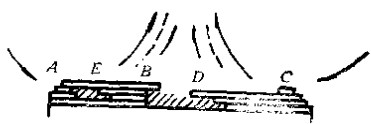
\includegraphics[width=0.7\textwidth]{fig/cp03/img3.34.jpg}
 \caption{晶面上过饱和度的差别($A$、$B$、$C>D$、$E$)破坏了生长的顺序性,造成母液包藏。}
\end{figure}

介质的运动对晶体生长速度和完整性都有显著的作用,这种作用往往又和过饱和度紧密联系在一起。介质运动由自然对流、强迫对流和晶体自身生长引起。对流是质量传输和热量传输的主要形式,它影响晶体生长动力学、杂质俘获、组分均匀性、形态稳定性和成核作用。一般来说,随着对流的增大晶体生长速度也增大,直到以生长动力学机制决定生长速度。在无对流的情况下,过饱和度的分布在晶面中心最低,棱边次之,隅角顶点最高。这种分布在过饱和度增大时更为突出,容易发生界面的不稳定,产生母液包藏。在水溶液晶体快速生长中,要求过饱和度和溶液相对于晶体的流苏都很大,使晶体生长机制进入动力学和扩散同时起作用。晶体正反方向转动可以减弱顺着晶体产生的“尾流”,防止母液包藏。溶液的充分搅拌可使整体溶液浓度和温度分布均匀,这对大晶面的稳定生长和防止大生长体系中的自发成核特别重要。
